\graphicspath{{notes/8cardinality/}}

\section{Cardinalities of Infinite Sets}\label{sec:card}

\iffalse

\subsection{Cantor's Notion of Cardinality}\label{subsec:cant}

During the late 1800's a German mathematician named Georg Cantor almost single-handedly overturned the foundations of mathematics. Prior to Cantor, mathematicians had understood a set to be nothing more than a collection of objects. Via the consideration of certain infinite sets (in particular his \hyperref[ex:cantor]{middle third set}), Cantor showed this naïve idea to be woefully inadequate. Cantor met great resistance from many famous mathematicians and philosophers who felt his ideas to be unnatural. He even managed to inflame several religious scholars who believed his investigation of infinity to be an affront to the divine! Despite strong initial antipathy, Cantor's notion of cardinality is now universally accepted by mathematicians. More importantly, by exposing the contradictions inherent in contemporary set theory, he convinced mathematicians that a rigorous axiomatic approach was necessary. The result was a revolution in foundational mathematics, now known as \emph{axiomatic set theory.} Indeed, Cantor's legacy is arguably the modern axiomatic nature of pure mathematics, where rigor dominates and mathematicians are obliged to follow logic wherever it leads, regardless of the bizarre paradoxes which might appear.\\

In this chapter we consider the basics of Cantor's contribution, essentially his extension of the concept of \emph{cardinality} to infinite sets.\\

Recall that if $A$ is a \emph{finite} set, then $\nm A$, the cardinality of $A$, is simply the number of elements in  $A$. This definition obviously does not extend to infinite sets. However, cardinality has a stronger purpose than merely attaching a number to each set: it can be viewed as a \emph{relation} and used to \emph{compare} sets. It is this interpretation that turns out to apply to infinite sets. For example, suppose that
\[A=\{\text{fish},\text{dog}\},\quad\text{and}\quad B=\{\alpha,\beta,\gamma\}.\]
Even though the elements of the sets $A$ and $B$ are completely different, we may use cardinality to compare the sizes of $A$ and $B$: since $\nm A=2$ and $\nm B=3$, we may write $\nm A<\nm B$ to indicate that $B$ has more elements as $A$: colloquially, ``$B$ is larger than $A$.''\\

It is at this point that Cantor enters the discussion. By Theorem \ref{thm:finitecard} and Corollary \ref{cor:finitecard}, the condition $\nm A<\nm B$ is equivalent to the existence of an injective (one-to-one) function $f:A\to B$ and the non-existence of a bijection $g:A\to B$. For example, the function $f:A\to B$ defined by
\[\text{fish}\longmapsto\alpha,\qquad\text{dog}\longmapsto\beta,\]
is clearly injective. In a sense, Theorem \ref{thm:finitecard} tells us how to compare the cardinalities of finite sets \emph{without} counting their elements. Cantor's seemingly innocuous idea was to turn this \emph{theorem} for finite sets into a \emph{definition} of cardinality for all sets.\pagebreak[4]

\begin{defn}\label{defn:infcard}
The \emph{cardinalities} of two sets $A,B$ are denoted $\nm A$ and $\nm B$. We compare cardinalities as follows:
\begin{itemize}
  \item $\nm A\le\nm B\iff\exists f:A\to B$ injective.
  \item $\nm A=\nm B\iff\exists f:A\to B$ bijective.
\end{itemize}
We write $\nm A<\nm B\iff \nm A\le \nm B$ and $\nm A\neq \nm B$. That is $\exists f:A\to B$ injective but $\nexists g:A\to B$ bijective.
\end{defn}

\noindent Cardinality is defined as an abstract \emph{property} whereby two sets can be \emph{compared.} Otherwise said, it is a \emph{relation.} To define a cardinality $\nm A$ as an object, we need the following theorem.

\begin{thm}\label{thm:cardequiv}
On any collection of sets, the relation $A\sim B\iff\nm A=\nm B$ is an equivalence relation.
\end{thm}

\noindent The cardinality of a set $A$ can then be defined to be the equivalence class of $A$ with respect to this relation: $\nm A:=[A]$. It is now clear that cardinality partitions any collection of sets: every set has a cardinality, and no set has more than one cardinality. We can moreover identify the cardinalities of finite sets with the cardinal numbers $0,1,2,3,4,\ldots$ in a natural way. To get further it is useful to introduce a symbol for the cardinality of the simplest infinite set.

\subsubsection*{Countably Infinite Sets}

\begin{defn}
The cardinality of the set of natural numbers $\N$ is denoted $\aleph_0$, read \emph{aleph-nought} or \emph{aleph-null.} We say that a set $A$ is \emph{countably infinite,} or \emph{denumerable}\footnote{Sometimes this is shortened to \emph{countable,} although some authors use countable to mean `finite or denumerable,' i.e. any $A$ for which $\nm A\le\aleph_0$. Use \emph{countably infinite} or \emph{denumerable} to avoid confusion. $\aleph$ is the first letter of the Hebrew alphabet.} if $\nm A=\aleph_0$.
\end{defn}

\noindent We will discuss in a moment why we need a new symbol, why $\infty$ doesn't suffice. First we consider an example of Definition \ref{defn:infcard} at work.

\begin{example}
Let $2\N=\{2,4,6,8,10,\ldots\}$ be the set of positive even integers. The function
\[f:\N\to 2\N:n\mapsto 2n\]
is a bijection. It follows that $\nm{2\N}=\nm\N=\aleph_0$ and we say that $2\N$ is denumerable.
\end{example}

\noindent This example immediately demonstrates one of strange properties of infinite sets: $2\N$ is a \emph{proper subset} of $\N$, and yet the two sets are in bijective correspondence with one another! You should feel like you want to say two contradictory things simultaneously:
\begin{itemize}
  \item $\N$ has the same `number of elements' as $2\N$.
  \item $\N$ has twice the `number of elements' as $2\N$.
\end{itemize}
If this doesn't make you feel uncomfortable, then read it again! The remedy to your discomfort is to appreciate that \emph{cardinality} and \emph{number of elements} are different concepts. Replacing `number of elements' with `cardinality' in the two statements makes both true! Indeed it is completely legitimate to write $2\aleph_0=\aleph_0$. The idea of a set having a proper subset with the same cardinality can be used as a \emph{definition} of infinite set (see Exercise \hyperref[ex:cardinf]{\ref*{subsec:cant}.\ref*{ex:cardinf}}).\\

Here is another example of the same phenomenon; $\N$ has one more element than $\N_{\ge 2}$ and yet they have the same cardinality: $\aleph_0+1=\aleph_0$.

\begin{example}
The function $g:\N\to\N_{\ge 2}:n\mapsto n+1$ is a bijection, whence $\N_{\ge 2}=\{2,3,4,5,\ldots\}$ is denumerable.
\end{example}



\paragraph{Proving that a set is denumerable}

While it is possible to use any number of clever theorems to prove the denumerability of a set $A$, the simplest thing to imagine listing the elements in some order so that $A$ `looks like' the natural numbers, or some other known denumerable set. For instance, the above examples can be summarized by listing the elements of these sets below those of the natural numbers:
\[\begin{array}{c||ccccccccccc}
\N&1&2&3&4&5&6&7&8&9&10&\cdots\\\hline\hline
2\N&2&4&6&8&10&12&14&16&18&20&\cdots\\\hline
\N_{\ge 2}&2&3&4&5&6&7&8&9&10&11&\cdots
\end{array}\]
The required bijective functions are then easy to read off! We use this technique to construct bijections which show the denumerability of two important examples.

\begin{thm}\label{thm:zcount}
The integers $\Z$ are denumerable.
\end{thm}

\begin{proof}
We must construct a bijective function $f:\N\to\Z$. By experimenting with listing the integers, we write down the first few terms of a suitable function in tabular form:
\[\begin{array}{c|ccccccccccc}
n&1&2&3&4&5&6&7&8&9&10&\cdots\\\hline
f(n)&0&1&-1&2&-2&3&-3&4&-4&5&\cdots
\end{array}\]
Two things should be clear from the table:
\begin{description}
\item[Surjectivity]\quad Every integer appears at least once in the second row.
\item[Injectivity]\quad No integer appears more than once in the second row.
\end{description}
It follows that the function $f$ is bijective.
\end{proof}

\noindent You might object that the above argument is too quick, and perhaps you don't trust the reasoning. Does the table really define a function? Is it really obvious that the function is bijective? We can be more formal and explicit, but the cost is that the big picture becomes less clear. Our function may be written
\[f(n)=\begin{cases}
\frac 12n&\text{if $n$ is even,}\\
-\frac 12(n-1)&\text{if $n$ is odd.}
\end{cases}\]
Now we check that this is bijective:\\[-5pt]

\noindent(\emph{Injectivity})\quad Let $m,n\in\N$, and suppose that $f(m)=f(n)$. Without loss of generality, there are three cases to consider.
\begin{ptabular}{(\emph{$m$ even, $n$ odd})}
(\emph{$m,n$ both even})&$f(m)=f(n)\implies \frac m2=\frac n2\implies m=n$.\\
(\emph{$m,n$ both odd})&$f(m)=f(n)\implies-\frac 12(m-1)=-\frac 12(n-1)\implies m=n$.\\
(\emph{$m$ even, $n$ odd})&$f(m)=f(n)\implies\frac m2=-\frac 12(n-1)\implies m+n=1$. But $m,n\in\N$, so $m+n\ge 2$, which is a contradiction.
\end{ptabular}
Therefore $f$ is injective.\\[-5pt]

\noindent(\emph{Surjectivity})\quad With a little calculation, you should be able to see that, for any $z\in\Z$, there exists a positive integer $n$ such that $f(n)=z$, namely:
\[z=\begin{cases}
f(2z)&\text{if $z>0$,}\\
f(1-2z)&\text{if $z\le 0$.}
\end{cases}\]
Hence $f$ is surjective.\\

\noindent For basic examples you are encouraged to use the listing/pictorial construction rather than explicitly writing everything out. Training your intuition is more important than the formality here! Indeed we would likely have been unable to come up with an explicit formula for $f$ without the table, and it is easier to get a feel for what $f$ is using the table rather than the formula.\\

As you build up examples, you no longer have to compare denumerable sets directly to the natural numbers. A set $B$ is denumerable if and only if $\exists f:A\to B$ bijective where $A$ is \emph{any denumerable set.} This holds because the composition of bijective function is also bijective (Theorem \ref{thm:compinjsurj}). For instance, we immediately see that the set of even integers $2\Z$ is denumerable because
\[f:\Z\to 2\Z:z\mapsto 2z\]
is a bijection, and because we now know that $\Z$ is denumerable. We use this approach to help prove the following result, the first of Cantor's truly counter-intuitive revelations.

\begin{thm}\label{thm:qcount}
The rational numbers $\Q$ are denumerable.
\end{thm}

\noindent We prove the Theorem in stages. First we construct a bijection between the natural numbers $\N$ and the positive rational numbers $\Q^+$. We then modify this to obtain a bijection between the integers $\Z$ and the full set of rational numbers $\Q$. By the previous Theorem, it follows that $\Q$ must be denumerable.

\begin{proof}
For each pair of natural numbers $a,b$, place the fraction $\frac ab\in\Q^+$ in the $a$th column and $b$th row of an infinite square as shown below. Now list the positive rational numbers by tracing the diagonals as shown, deleting any number that has already appeared in the list ($\frac 22=\frac 11$, \ $\frac 64=\frac 32$, etc.).
\begin{center}
\begin{minipage}{0.38\textwidth}\centering
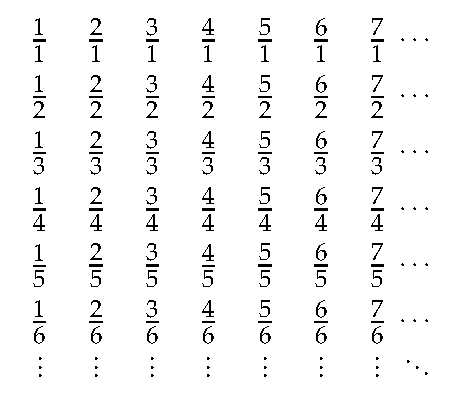
\includegraphics[width=\textwidth]{cardinality-01-qcount}\\
The infinite square
\end{minipage}\qquad\qquad\qquad
\begin{minipage}{0.38\textwidth}\centering
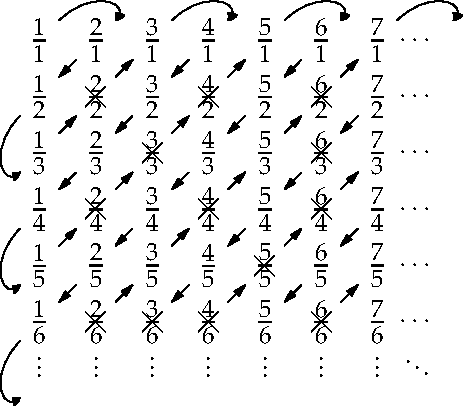
\includegraphics[width=\textwidth]{cardinality-02-qcount}\\
Trace diagonals and delete repeats
\end{minipage}
\end{center}
We obtain the \emph{ordered set}
\[\{a_1,a_2,a_3,a_4,\ldots\}=\left\{{\frac 11,\,\frac 21,\,\frac 12,\,\frac 13,\,\frac 31,\,\frac 41,\,\frac 32,\,\frac 23,\,\frac 14,\,\frac 15,\,\ldots}\right\}.\]
Now define the function $f:\N\to\Q^+$ by $f(n)=a_n$. This is certainly a function. We claim that it is a bijection.\\[-5pt]

\noindent(\emph{Injectivity})\quad Let $m,n\in\N$, and suppose that $f(n)=f(m)$. Then $a_m=a_n$. In the above construction we deleted any rational number which had already appeared in the list. Thus $a_m$ can only equal $a_n$ if $m=n$.\\[-5pt]

\noindent(\emph{Surjectivity})\quad A positive rational number $\frac ab$ appears in the $a$th column and $b$th row of the square (and in many other places, $\frac ab=\frac{2a}{2b}=\cdots$). We only delete a fraction $\frac ab$ if it has already appeared in the list, therefore every positive rational lies in the range of $f$.\\[-5pt]

\noindent To finish things off, we extend the function to all rational numbers by
\[g:\Z\to\Q:n\mapsto\begin{cases}
f(n)&\text{if }n>0,\\
0&\text{if }n=0,\\
-f(-n)&\text{if }n<0.
\end{cases}\]
We are merely using $f$ to identify the negative integers with the negative rationals. It is immediate that $g:\Z\to\Q$ is a bijection. Appealing to Theorem \ref{thm:zcount}, we deduce that $\nm{\Q}=\nm{\Z}=\aleph_0$, and so $\Q$ is denumerable.
\end{proof}

\noindent This result should surprise you! Any sensible person should feel that there are far, far more rational numbers than integers, and yet the two sets have the same cardinality. Bizarre.\\

There are other denumerable sets that appear to be even larger than $\Q$. For example, we can show that the Cartesian product $\N\times\N$ is denumerable: use almost the same proof as for $\Q^+$ except that there are no repeats to delete. For a much larger-seeming yet still denumerable set, consider the \emph{algebraic numbers:}
\[\big\{x\in\R:p(x)=0\text{ for some polynomial $p$ with integer coefficients}\big\}.\]
Algebraic numbers are the zeros of polynomials with integer coefficients. Clearly any rational number $\frac ab$ is algebraic, since it satisfies $p(x)=0$ for $p(x)=bx-a$. There are many more algebraic numbers than rational numbers: e.g. $\sqrt[5]{2}-3$ is algebraic since it is a root of the polynomial $p(x)=(x+3)^5-2=0$. Not all real numbers are algebraic however: those which aren't, such as $\pi$ and $e$, are termed \emph{transcendental.}

\subsubsection*{The least infinite cardinal?}

We originally introduced the symbol $\aleph_0$ to represent the cardinality of the `simplest' infinite set. While the natural numbers are certainly infinite and straightforward, is there any more compelling reason why we should consider them to be the \emph{most simple} infinite set? One reason lies in the following result.

\begin{thm}\label{thm:finitealeph}
$A$ is a finite set if and only if $\nm A<\aleph_0$.
\end{thm}

\noindent Otherwise said, every infinite set has cardinality \emph{at least as large} as the natural numbers: $\aleph_0$ may be considered the least infinite cardinal.

\begin{proof}
($\Longrightarrow$)\quad The $n=0$ case is left to the Exercises. Suppose that $\nm A=n\ge 1$ so that we may list the elements of $A$ as $\{a_1,\ldots,a_n\}$. We must prove two things:
\begin{enumerate}
  \item $\nm A\le\aleph_0$. That is, $\exists f:A\to\N$ which is \emph{injective.}
  \item $\nm A\neq\aleph_0$. That is, $\nexists g:A\to\N$ which is \emph{bijective.} By symmetry this is equivalent to showing that there is no bijective function $h:\N\to A$.\footnote{If $g:A\to\N$ is a bijection, then $g^{-1}:\N\to A$ is also a bijection.}
\end{enumerate}
For part 1., simply define $f$ by $f(a_k)=k$ for each $k\in\{1,2,3,\ldots,n\}$. This is injective since the distinct elements $a_k$ of $A$ map to distinct integers.\\
For part 2., suppose that $h:\N\to A$ is bijective. Consider the set
\[h\bigl(\{1,\ldots,n+1\}\bigr)=\bigl\{h(1),\ldots,h(n+1)\bigr\}\subseteq A.\]
Since $A$ has $n$ elements, by Dirichlet's box principle, at least two of the values $h(1),\ldots,h(n+1)$ must be equal. Therefore $h$ is not injective and consequently not bijective. A contradiction.\\[3pt]
($\Longleftarrow$)\quad See Exercise \hyperref[ex:cardinf]{\ref*{subsec:cant}.\ref*{ex:cardinf}.}
\end{proof}

\noindent Of course, this doesn't answer the question of whether there exist infinite sets with larger cardinality than $\aleph_0$, though we shall answer this in the next section.

\begin{aside}
\noindent{\bf $\aleph_0$ versus $\infty$: what's the difference?}

It can be difficult to grasp why $\aleph_0$ and $\infty$ are not the same thing. The problem is compounded by references to an `infinite number' of objects whenever the cardinality of a set is not finite. This loose phrase is commonly used, but risks conflating the concepts of `infinite set' and `infinity.'\\
So what is the difference between $\aleph_0$ and $\infty$? If there aren't an `infinite number' of natural numbers, how many are there? Theorem \ref{thm:finitealeph} says that $\aleph_0$ is `larger than any natural number.' Is this not what we mean by infinity? The reason we need a new symbol $\aleph_0$, and why it and $\infty$ are different, is twofold:
\begin{enumerate}
\item As we shall see shortly, there are infinite sets with greater cardinality than $\aleph_0$: in a naïve sense, there are multiple infinities. The single symbol $\infty$ is insufficient to distinguish sets with different infinite cardinalities.
\item More philosophically, $\aleph_0$ is an \emph{object} in its own right; an object to which the cardinality of some set may be equal. Indeed, by Theorem \ref{thm:cardequiv}, $\aleph_0$ is an equivalence class.

By contrast, $\infty$ is typically not an object. The symbol $\infty$ is mostly used in \emph{interval notation} and when talking about \emph{limits:} in neither case does the symbol represent an object. For example:
\begin{itemize}
  \item The interval $(2,\infty)$ is the set of all real numbers greater than 2. We don't say `greater than 2 and \emph{less than infinity.}'
  \item $\lim\limits_{x\to 3}\frac 1{(x-3)^2}=\infty$ means that the function $f(x)=\frac 1{(x-3)^2}$ gets unboundedly larger as $x$ approaches 3. It is incorrect to say that $f(x)$ `approaches infinity.' It is even worse to write $f(3)=\frac 1{(3-3)^2}=\infty$.
\end{itemize}
\end{enumerate}

\noindent The challenge of Cantor's notion of cardinality is to appreciate that the question, `How many natural numbers are there?' is meaningless!
\end{aside}

\paragraph{Self-test Questions}

\begin{enumerate}
  \item A set $A$ is \emph{denumerable} if \underline{\phantom{there exists a bijection $f:A\to\N$\qquad\qquad}}
  
  \item True or false: if $A$ is a proper subset of $B$, then $A$ has smaller cardinality than $B$.
\end{enumerate}

\subsection*{Exercises}

\begin{enumerate}\renewcommand{\labelenumi}{\thesubsection.\theenumi}
  \item Refresh your proof skills by proving explicitly that the following functions are bijections:
  \begin{enumerate}
    \item $f:\N\to 2\N:n\mapsto 2n$.
    \item $g:\N\to\N_{\ge 2}:n\mapsto n+1$.
  \end{enumerate}
  
	\item Construct a function $f:\N\to\Z_{\ge -3}=\{-3,-2,-1,0,1,2,3,4,\ldots\}$ which proves that the latter set is denumerable: you must show that your function is a bijection.
	
  \item Prove that the set $3\Z+2=\{3n+2:n\in\Z\}$ is denumerable.
	
	\item Show that the set of all triples of the form $(n^2,5,n+2)$ with $n\in 3\Z$ is denumerable by explicitly providing a bijection with a denumerable set $A$. (\emph{You must check that the set $A$ is denumerable, and that your map is indeed a bijection.})

	\item Imagine a hotel with an infinite number of rooms: Room 1, Room 2, Room 3, Room 4, etc.. Show that, even if the hotel is full, the guests may be re-accommodated so that there is always a room free for one additional guest.\\
\emph{Hint: consider the function $f:\N\to\N:n\mapsto n+1$.}
	
	\item Prove that $A\subseteq B\Longrightarrow \nm A\le\nm B$. (\emph{You need an injective function $f:A\to B$})
		
	\item Prove Theorem \ref{thm:cardequiv}. (\emph{You need little more than Theorem \ref{thm:compinjsurj} on the composition of bijective functions.})

	\item Prove that the set $\N\times\N$ is denumerable. You should base your proof on Theorem \ref{thm:qcount}.

	\item We know that $\Q$ is denumerable, and we saw (Theorem \ref{thm:qcount}) that there must exist a bijective function $f:\N\to\Q$. Show that $g:\N\times\N\to\Q\times\Q$ defined by $g(m,n)=(f(m),f(n))$ is a bijection. Appeal to the previous question to show that $\Q\times\Q$ is denumerable.
	
	\item Here we consider the $n=0$ case of Theorem \ref{thm:finitealeph}. Recall the definition of function in Section \ref{sec:func2}.
  \begin{enumerate}
    \item If $\nm A=0$, then $A=\emptyset$. Suppose that $f:\emptyset\to\N$ is a function. Use Definition \ref{defn:func} to prove that $f=\emptyset$.
    \item State what it means, in the language of Definition \ref{defn:func}, for a function $f:A\to\N$ to be injective. Show that $f=\emptyset$ is an injective function.
    \item Suppose that $B$ is a set with $\nm B\ge 1$. Prove by contradiction that there are no functions $h:B\to\emptyset$. Conclude that $0<\aleph_0$.
  \end{enumerate}

	\item\label{ex:cardunion} Suppose that the set $A_n$ is denumerable for each $n\in\N$. We may then list the elements of each set: $A_n=\{a_{n1},a_{n2},a_{n3},a_{n4},\ldots\}$. Now list the elements of the sets $A_1,A_2,A_3,\ldots$ as follows:
	\begin{gather*}
		A_1=\{a_{11},a_{12},a_{13},a_{14},\ldots\}\\
		A_2=\{a_{21},a_{22},a_{23},a_{24},\ldots\}\\
		A_3=\{a_{31},a_{32},a_{33},a_{34},\ldots\}\\
		\qquad\vdots
	\end{gather*}
	Use this construction to prove that $\bigcup\limits_{n\in\N}A_n$ is a denumerable set.\\
	\emph{This result is often stated, `A countable union of countable sets is countable.'}
	
	\item(Hard!) In this question we complete the proof of Theorem \ref{thm:finitealeph} by showing that if $\nm A<\aleph_0$, then $A$ is a finite set.\\[2pt]
	We prove by contradiction. Suppose that $A$ is an infinite set such that $\nm A<\aleph_0$. Then there exists an injective function $f:A\to\N$. List the elements of the image of $f$ in increasing order:
	  \[\range(f)=\{n_1,n_2,n_3,\ldots\}.\]
	\begin{enumerate}
	  \item Prove that $\im f$ is an infinite set.
	  \item Show that for all $k\in\N$, there exists a unique $a_k\in A$ satisfying $f(a_k)=n_k$.
	  \item Define $g:\N\to A$ by $g(k)=a_k$. Prove that $g$ is a bijection.
	  \item Why do we obtain a contradiction?
	\end{enumerate}
	
	\item\label{ex:cardinf} Prove that a set $A$ is infinite if and only if it has a proper subset $B\subset A$ with the same cardinality $\nm B=\nm A$.
\end{enumerate}
\newpage

\subsection{Uncountable Sets}


Since $\Q$ seems so large, you might think that there cannot be any sets with strictly larger cardinality. But we haven't yet thought about the real numbers\ldots

\begin{defn}
A set $A$ is \emph{uncountable} if $\nm A>\aleph_0$, that is if there exists an injection $f:\N\to A$ but no bijection $g:\N\to A$.
\end{defn}

\begin{thm}
The interval $[0,1]$ of real numbers is uncountable.
\end{thm}

\noindent We denote the cardinality of the interval $[0,1]$ by the symbol $\fc$ for \emph{continuum.} The theorem may therefore be written $\fc>\aleph_0$.

\begin{proof}
First we require an injective function $f:\N\to[0,1]$. The function defined by $f(n)=\frac 1n$ clearly fits the bill, for
\[f(n)=f(m)\implies \frac 1n=\frac 1m\implies n=m.\]
Now we prove that there exists no bijection $g:\N\to[0,1]$, arguing by contradiction. Suppose that $g$ is such a bijection and consider the sequence of values $g(1),g(2),g(3),\ldots$ These are real numbers between 0 and 1, hence they may all be expressed as decimals:\footnote{A number has two decimal representations if and only if one of them terminates and the other ultimately becomes an infinite sequence of 9's. For the purposes of this proof it does not matter which representation is chosen when there is a choice. We are forced, however, to take $1=0.999999\cdots$, due to our insistence that all elements be written with zero units.}
\[\begin{array}{c}
g(1)=0.b_{11}b_{12}b_{13}b_{14}b_{15}b_{16}\cdots\\[2pt]
g(2)=0.b_{21}b_{22}b_{23}b_{24}b_{25}b_{26}\cdots\\[2pt]
g(3)=0.b_{31}b_{32}b_{33}b_{34}b_{35}b_{36}\cdots\\[2pt]
g(4)=0.b_{41}b_{42}b_{43}b_{44}b_{45}b_{46}\cdots\\[2pt]
g(5)=0.b_{51}b_{52}b_{53}b_{54}b_{55}b_{56}\cdots\\[-2pt]
\vdots\\[-8pt]
\end{array}\qquad\text{where each }b_{ij}\in\{0,\ldots,9\}.\]
Since $g$ is bijective, it is certainly surjective. It follows that all of the values $c\in[0,1]$ appear in the above list of decimals. Now define a new decimal
\[c=0.c_1c_2c_3c_4c_5\cdots\qquad\text{where}\quad c_n=\begin{cases}
1&\text{if }b_{nn}\neq 1,\\
2&\text{if }b_{nn}=1.
\end{cases}\]
$c$ is a non-terminating decimal whose digits are 1's and 2's, whence it has no other representation. Since $c$ disagrees with $g(n)$ at the $n$th decimal place, we have $c\neq g(n),\ \forall n\in\N$. Hence $c$ is \emph{not} in the above list. However $c\in[0,1]$ and $g$ is surjective, whence $c\neq g(n)$ for some $n\in\N$: a contradiction. We conclude that $\fc\neq\aleph_0$.\\
Putting this together with the first part of the proof where $\fc\ge\aleph_0$, we conclude that $\fc>\aleph_0$.
\end{proof}

\noindent The second part of the proof is known as \emph{Cantor's diagonal argument,} since we are comparing the constructed decimal $c$ with the diagonal of an infinite square of integers. We have proved that the interval $[0,1]$ has a strictly larger cardinality than the set of integers. Since $[0,1]\subseteq\R$, it follows immediately that the real numbers are also uncountable. Indeed we shall see in a moment that the real numbers also have cardinality $\fc$, as does any interval (of positive width). More amazingly, the Cantor middle-third set (page \pageref{ex:cantor}) also has cardinality $\fc$, despite seeming vanishingly small.

\subsubsection*{More advanced ideas}

Our countable and uncountable examples are merely scratching the surface of a truly weird subject. We conclude these notes with a couple more ideas.\\

The following theorem is very useful for being able to compare cardinalities. It allows us to prove that two sets have the same cardinality \emph{without} explicitly constructing bijective functions. Injective functions are usually much easier to find.

\begin{thm}[Cantor--Schröder--Bernstein]
If $\nm A\le\nm B$ and $\nm B\le\nm A$, then $\nm A=\nm B$.
\end{thm}

\noindent The theorem seems like it should be obvious, but pause for a moment: it is \emph{not} a result about \emph{numbers!} $A$ and $B$ are \emph{sets,} and so the theorem must be understood in the context of Definition \ref{defn:infcard}. In this language the theorem becomes:
\begin{quote}
Suppose there exist \emph{injective} functions $f:A\to B$ and $g:B\to A$.\\
Then there exists a \emph{bijective} function $h:A\to B$.
\end{quote}
The proof is beautiful, though a little long to reproduce here. If you are interested it can be found in any text on set theory. The applications of the theorem are more important to our purposes.

\begin{thm}
The interval $(0,1)$ has cardinality $\fc$.
\end{thm}

\noindent It is possible to explicitly define a bijection $h:(0,1)\to[0,1]$, although it is very messy. Instead we construct two injections.

\begin{proof}
$f:(0,1)\to[0,1]:x\mapsto x$ is clearly an injection, whence $\nm{(0,1)}\le\nm{[0,1]}=\fc$. Now define
\[g:[0,1]\to (0,1):x\mapsto \frac 12x+\frac 14.\]
$g$ is certainly injective, and so $\fc\le\nm{(0,1)}$.\\[2pt]
By the Cantor--Schr\"oder--Bernstein Theorem, the sets $(0,1)$ and $[0,1]$ have the same cardinality $\fc$.
\end{proof}

\noindent In case you're feeling nervous, note that the function $g$ in the proof isn't surjective: the range of $g$ is the interval $[\frac 14,\frac 34]\neq (0,1)$. By a similar trick, covered in the Exercises, one can see that $\R$ also has cardinality $\fc$.\\

For a final punchline, we prove Cantor's Theorem, which says that the power set of any set $A$ always has a strictly larger cardinality than $A$. In Theorem \ref{thm:powercard} we saw that $\nm{\cP(A)}=2^{\nm A}$ for finite sets $A$. We therefore already believe that Cantor's Theorem is true for finite sets. The proof that follows also works for infinite sets.

\begin{thm}[Cantor]
If $A$ is any set, then $\nm A\lneq\nm{\cP(A)}$.
\end{thm}

\begin{proof}
If $A=\emptyset$, the result is trivial. Otherwise, we must show two things:
\begin{itemize}
  \item $\exists f:A\to\cP(A)$ which is injective.
  \item $\nexists g:A\to\cP(A)$ which is bijective.
\end{itemize}
For the first, note that $f:a\mapsto\{a\}$ is a suitable injective function.\\
Now suppose for a contradiction that $\exists g:A\to\cP(A)$ which is bijective. That is, $g(a)$ is a subset of $A$ for each $a\in A$. Consider the set
  \[X=\{a\in A:a\not\in g(a)\}.\]
  It is important to note that $X$ \emph{is a subset of $A$.}\phantom\qedhere
\end{proof}
  
\noindent We pause the proof for a moment, as the set $X$ is somewhat tricky to think about. Before proceeding, let us consider an example. Suppose that $g:\{1,2\}\to\cP(\{1,2\})$ is defined by
  \[g(1)=\{1,2\},\qquad g(2)=\{1\}.\]
  Then $1\in g(1)$ and $2\not\in g(2)$, whence the above set is $X=\{2\}$. Since we are trying to prove that no bijection $g:A\to\cP(A)$ exists, it is important to note that the function $g$ in our example is \emph{not bijective!}

\begin{proof}[Proof Continued]  
By assumption, $g$ is bijective, hence it is certainly surjective. Because the range of $g$ is the power set $\cP(A)$, the set \emph{$X$ lies in the image of $g$.} Otherwise said, there exists $b\in A$ such that $g(b)=X$. We ask whether $b$ is an element of $X$. Think carefully about the definition of $X$, and observe that
\begin{align*}
b\in X&\iff b\not\in g(b)\tag*{(by the definition of $X$)}\\
&\iff b\not\in X\tag*{(since $X=g(b)$)}
\end{align*}
Look at what we have concluded: $b\in X\iff b\not\in X$. This is clearly a contradiction!\\[2pt]
It follows that there exists no bijection $g:A\to\cP(A)$, and so $\nm A\lneq\nm{\cP(A)}$.
\end{proof}

\noindent The main implication of this is that \emph{there is no largest cardinality!} We can always construct a larger set simply by taking the power set of what we already have. For example, $\cP(\R)$ has larger cardinality than $\R$. If you want a set with even larger cardinality, why not take $\cP(\cP(\R))$? Or $\cP(\cP(\cP(\R)))$. We can continue this process indefinitely.

Cantor's Theorem played a large part in pushing set theory towards axiomatization. Here is a conundrum motivated by the theorem: If a `set' is just a collection of objects, then we may consider the `set of all sets.' Call this $A$. Now consider the power set of $A$. Since $\cP(A)$ is a set of sets, it must be a subset of $A$, whence $\nm{\cP(A)}\le\nm A$. However, by Cantor's Theorem, we have $\nm A\lneq\nm{\cP(A))}$. The conclusion is the manifest absurdity
\[\nm{A}\lneq\nm{A}\]
The remedy is a thorough definition of `set' which prevents the collection of all sets from being considered a set. This is where \emph{axiomatic set theory} begins. 


% \begin{proof}
% We are assuming that we have two distinct, injective functions $f:A\to B$ and $g:B\to A$. We must construct a bijective $h:A\to B$.
% 
% Consider some $\alpha\in A$. Does $\exists\beta\in B$ such that $\alpha=g(\beta)$? If so, then the injectivity of $g$ says that $\beta$ is unique and we might as well write $\beta=g^{-1}(\alpha)$. Now suppose that $\exists\gamma\in A$ such that $\beta=f(\gamma)$. Again, if $\gamma$ exists, the injectivity of $f$ says it is unique and we can write $\gamma=f^{-1}(\beta)=f^{-1}(g^{-1}(\alpha))$.
% 
% Starting with $\alpha\in A$, we ask how far we can continue this process of following the functions $g,f$ in reverse. Each $\alpha\in A$ must be one of two possible types:
% \begin{enumerate}
%   \item Type I: The process continues indefinitely, or will terminate in the set $A$: i.e. after an even number of steps, the chain results in some $a\in A$ which is \emph{not} in the image of $g$ and thus for which $g^{-1}(a)$ does not exist.
%   \item Type II: The process terminates in the set $B$.
% \end{enumerate}
% We now define the function that will turn out to be the required bijection: if $\alpha\in A$, define
% \[h(\alpha)=\begin{cases}
% f(\alpha)&\text{if $\alpha$ Type 1},\\ 
% g^{-1}(\alpha)&\text{if $\alpha$ Type 2}.
% \end{cases}\]
% 
% Is $h$ a well-defined function? There is no overlap between the two Types. Furthermore, if $\alpha$ is Type I, $f(\alpha)$ is always defined, while for Type 2, the we must be able to apply $g^{-1}$ at least once to $\alpha$. $h:A\to B$ is therefore well-defined.
% 
% We now prove that $h$ is a bijection.
% 
% Suppose $h(\alpha_1)=h(\alpha_2)$. There are three cases:
% \begin{enumerate}
% \item $\alpha_1,\alpha_2$ of Type 1. Then the injectivity of $f$ forces, 
% \[h(\alpha_1)=h(\alpha_2)\implies f(\alpha_1)=f(\alpha_2)\implies\alpha_1=\alpha_2.\]
% \item $\alpha_1,\alpha_2$ of Type 2. Then we apply $g$ to obtain, 
% \[h(\alpha_1)=h(\alpha_2)\implies g^{-1}(\alpha_1)=g^{-1}(\alpha_2)\implies\alpha_1=\alpha_2.\]
% \item $\alpha_1$ of Type 1 and $\alpha_2$ of Type 2. Then, 
% \[h(\alpha_1)=h(\alpha_2)\implies f(\alpha_1)=g^{-1}(\alpha_2)\implies \alpha_2= 
% g(f(\alpha_1).\]
% But this says that $\alpha_1$ and $\alpha_2$ have the same type. A contradiction.
% \end{enumerate}
% $h$ is therefore injective.\\
% 
% Now for surjectivity. Let $\beta\in B$. We want to find an $\alpha$ with $h(\alpha)=\beta$. Consider 
% the chain of $g(\beta)$. If $g(\beta)$ is of Type 1 then $f^{-1}(\beta)$ is well-defined and $h(f^{-1}(\beta))=\beta$. If instead $g(\beta)$ is of Type 2 then $h(g(\beta))=g^{-1}(g(\beta))=\beta$. Hence $h$ is onto.
% \end{proof}

\paragraph{Self-test Questions}

\begin{enumerate}
  \item A set $A$ is \emph{uncountable} if \underline{\phantom{there exists no injection $f:A\to\N$\qquad\qquad}}
  
  \item For each of the following sets, decide whether they are countable or uncountable.
  \[(1,2]\cup\{3\},\qquad \N\times[1,2],\qquad\R\setminus\left\{\tfrac 1n:n\in\N\right\},\qquad \Q\cap[1,2].\] 
\end{enumerate}

\subsection*{Exercises}

\begin{enumerate}\renewcommand{\labelenumi}{\thesubsection.\theenumi}
  \item You may assume that $[0,1]$ has cardinality $\fc$.
  \begin{enumerate}
    \item Construct an explicit bijection $f:[0,1]\to [3,8]$ which proves that the interval $[3,8]$ also has cardinality $\fc$. \emph{Try a linear function mapping the endpoints of $[0,1]$ to the endpoints of $[3,8]$.}
    \item Let $a,b\in\R$ with $a<b$. Generalizing part (a), construct a bijection which proves that the closed interval $[a,b]$ has cardinality $\fc$.
  \end{enumerate}
  
  \item\begin{enumerate}
    \item Suppose that $g:\{1,2,3,4\}\to\cP(\{1,2,3,4\})$ is defined by
  	\[g(1)=\{1,2,3\},\qquad g(2)=\{1,4\},\qquad g(3)=\emptyset,\qquad g(4)=\{2,4\}.\]
  	Compute the set $X=\bigl\{a\in\{1,2,3,4\}:a\not\in g(a)\bigr\}$.
  	\item Repeat part (a) for $g:\N\to\cP(\N):n\mapsto\{x\in 2\N:x\le n\}$.
  \end{enumerate}
  
   \item The proof of Cantor's Theorem makes use of a construction similar to \emph{Russell's Paradox.} Let $X$ be the set of all sets which are not members of themselves: explicitly
  	\[X=\{A:A\not\in A\}.\]
  	\begin{enumerate}
    	\item Assume that $X$ is a set, and use it to deduce a contradiction: ask yourself if $X$ is a member of itself.
    	\item Russell's paradox is one avatar of an ancient logical conundrum which appears in many guises. For example, suppose that a town has one hairdresser, and suppose that the hairdresser is the person who cuts the hair of all the people, and only those people, who do not cut their own hair. Who then cuts the hairdresser's hair? Can you explain the connection with Russell's paradox/Cantor's Theorem?
  	\end{enumerate}
  	\emph{The point of Russell's paradox is that we need a definition of `set' which prevents objects like $X$ from being considered sets.}
  
	\item Recall the Cantor set as described in the notes, where we proved that $\mathcal C$ is the set of all numbers in $[0,1]$ possessing a ternary expansion consisting only of zeros and twos. Modeling your answer on the proof that the interval $[0,1]$ is uncountable, prove that $\mathcal C$ is uncountable.
	
	\item Let $\mathbb I=\R\setminus\Q$ be the set of irrational numbers.
	\begin{enumerate}
	  \item Prove that $\nm{\mathbb I}\le\fc$.
	  \item Prove that $x\in\Q\implies x+\sqrt 2\in\mathbb I$. Hence conclude that $\aleph_0\le\nm{\mathbb I}$.
	  \item Appeal to Exercise \hyperref[ex:cardunion]{\ref*{subsec:cant}.\ref*{ex:cardunion}} to argue that the irrational numbers are uncountable.
 	\end{enumerate}
 	\emph{It is true, though we haven't show it, that $\nm{\mathbb I}=\fc$. Doing so is more difficult!}
  	
 	\item\begin{enumerate}
  		\item Prove that $f:\N\times\N\to\N$ defined by $f(m,n)=2^m3^n$ is injective.
  		\item Use part (a) and the Cantor--Schr\"oder--Bernstein Theorem to conclude that $\nm{\N\times\N}=\aleph_0$.
  		\item Extend your argument to conclude that, for any $k\in\N$,
  		\[\underbrace{\nm{\N\times\cdots\times\N}}_{k\text{times}}=\aleph_0\]
  		\item Use part (b) to provide an alternative proof that $\nm{\Q^+}=\aleph_0$.
  	\end{enumerate}
	
	\item\begin{enumerate}
  		\item Show that $\nm{(0,1)}\le\nm{\R\setminus\N}\le\nm{\R}$.
  		\item Construct a bijection $f:(0,1)\to (-\frac\pi 2,\frac\pi 2)$. (\emph{Try a linear function})
  		\item Show that $g:(-\frac\pi 2,\frac\pi 2)\to\R:x\mapsto\tan x$ is a bijection.
  		\item Use the Cantor--Schr\"oder--Bernstein Theorem to conclude that $\nm{\R\setminus\N}=\nm{\R}=\fc$.
  	\end{enumerate}
  	
  		
	\item (Hard!) Let $x\in[0,1]$. The \emph{binary expansion} of $x$ is the sequence $b_n$ of zeros and ones such that
  \[x=\sum_{n=1}^\infty \frac{b_n}{2^n}.\]
  Given the choice,\footnote{The binary expansion of $x$ is unique unless $x$ has a terminanting expansion, in which case the the other expansion involves an infinite sequence of ones: e.g. $[0.011111\cdots]_2=[0.1]_2$ in binary.} we choose the terminating binary expansion of $x$. With such a caveat, you are given that the binary expansion of $x\in[0,1]$ is unique. Define a function $f:[0,1]\to\cP(\N)$ by
  \[f(x)=\{n\in\N:b_n=1\text{ in the binary expansion of $x$}\}.\]
  \begin{enumerate}
    \item Prove that $f$ is an injection, and that, consequently, $\fc\le\nm{\cP(\N)}$.
		\item Prove that the function $g:\cP(\N)\to\mathcal C$ (the Cantor set) defined by
		\[g(X)=\sum\limits_{n\in X}^\infty\frac{2}{3^n}\]
		is a \emph{bijection.}
		\item Use Cantor--Schr\"oder--Bernstein to conclude that $\nm{\cP(\N)}=\nm{\mathcal C}=\fc$.
	\end{enumerate}
\end{enumerate}

\fi